% !TEX root = BA-Bauer

\subsection{Schaltungsprinzip}

In diesem Kapitel wird auf das grundsätzliche Prinzip der Schlatung eingegangen. Auf die einzelnen Komponenten und deren nötige Beschaltung wird in den folgenden Kapiteln eingegangen. Generell wird bei der Entwicklung der Schaltung darauf geachtet, dass möglichst keine fertigen Modulbausteine verwendet werden. Dadurch ergibt sich in der Regel ein Preisvorteil und das industrielle Bestücken einer Platine ist einfacher(Quelle?). (Abbildung verlinken)

\vspace*{5mm}
\begin{figure}[h]
	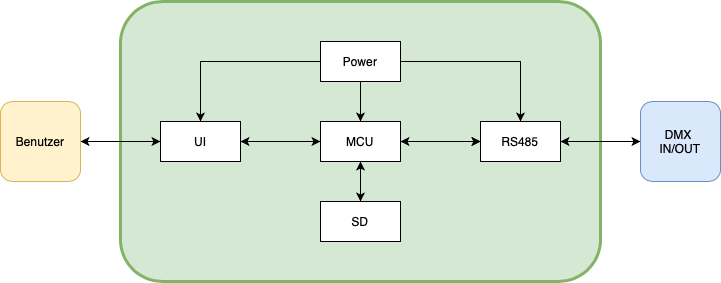
\includegraphics[width = \textwidth]{Schaltungsprinzip}
	\caption{Schaltungsprinzip}
	\label{fig:Schaltungsrinzip}
\end{figure}
\hspace*{-5mm}\textbf{Mikrocontroller (MCU)}\\
Der MCU bildet das Herzstück der Schaltung, über den sämtliche Kommunikation für die Benutzerschnittstelle, den DMX-Ein- und Ausgang und die SD-Karte läuft. Aufrgund der hohen Anforderungen wird hier bei der Entwicklung ein besonderes Augenmerk gelegt. Die Auswahl des MCUs richtet sich an dem in der vorangegangen Praxisprojektarbeit verwendeten Mikrocontroller. Auswahlkriterien sind eine mindestens gleichhohe Taktfrequenz des Prozessors, eine verfügbare UART-Schnittstelle, eine SDIO-Schnittstelle und mindestens drei Timer.\\
\textbf{Spannungsversorgung (Power)}\\
Die Spannungsversorgung für alle Komponenten wird von einer USB Schnittstelle geliefert, welche keine Daten übertragt. Über die USB-Schnittstelle werden 5V geliefert (Quelle), welche dann in enstprechend benötigte Spannungen gewandelt werden. Besonders kritisch ist die Versorgung des Mikrocontrollers. Unter normalen Betriebsbedingungen darf die Versorgungsspannung nur soweit einbrechen, dass der Mikrocontroller weiterhin das darauf installierte Programm ausführen kann.\\
\textbf{Benutzerschnittstelle (UI)}\\
Damit der Benutzer das Gerät Bedienung kann ist ein Informationsfluss in zwei Richtungen eforderlich. Zum einen müssen Eingaben durch den Benutzer erfasst werden, zum anderen muss das Gerät dem Benutzer eine Rückmeldung ausgeben können. Für die Benutzereingaben werden Taster und ein Drehgeber (Encoder) verwendet. Durch den Einsatz von Tastern können präzise und zeitgenaue Eingaben vom Benuter vorgenommen werden, an Stellen an denen es nötig ist, zum Beispiel beim starten einer Wiedergabe. Der Encoder hingegen bietet die Möglichkeit viele Eingaben in kurzer Zeit zu tätigen, zum Beispiel wenn die Aufnahmezeit eingestellt wird.

////SD